\chapter{Conclusão} 

\section{Discussão dos Resultados} 

As classes destinadas à implementação da interface no framework android fornecem
acesso a recursos que servem para implementação de responsabilidades não
relacionadas com a interface. Essa característica do framework android leva à
implementação da camada de View com diversas responsabilidades que não são
inerentes à interação com o usuário. Isso dificultou a refatoração, pois as
classes que exercem o papel de Presenter necessitam interagir com as classes de
View para acessar esses recursos, além de atualizar o estado da View. O uso do
padrão de injeção de
dependência\footnote{Padrão
de projeto onde um objeto recebe as referências para as suas dependências sem
conhecer os processo de contrução das mesmas.
\url{http://en.wikipedia.org/wiki/Dependency_injection}}
pode ser aplicado para acessar esses recursos e serviços sem a necessidade de
interação com a classe de View. A figura \ref{fig:classes_iteracao3} mostra a
disposição das classes após a refatoração.


\begin{figure}[htb]
	\label{fig:classes_iteracao3}
	\caption{Pacote após refatoração}
	\begin{center}
		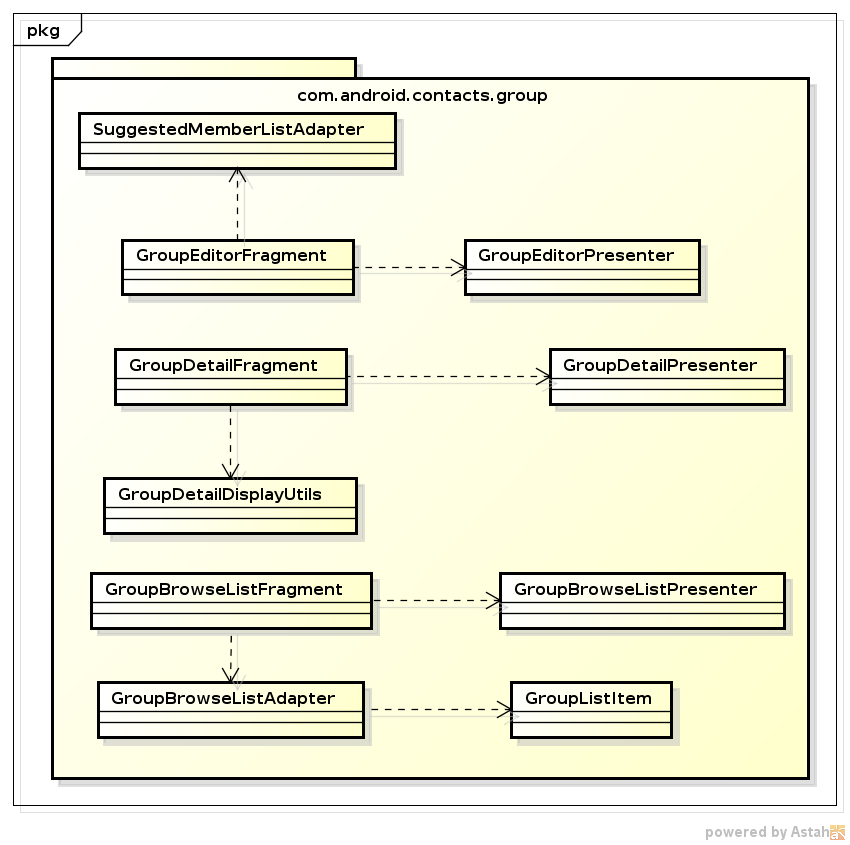
\includegraphics[scale=0.5]{img/classes_iteracao3}
	\end{center}
	\legend{Fonte: Próprio Autor}
\end{figure}


Ao usar o padrão MVP, a quantidade de linhas de métodos diminui pois cada um
dos componentes implementaram uma parte do caso de uso, aumentando o números de
métodos que se reflete na métrica WMC. Na implementação original onde um método
que era implementado na classe View, tinha a  responsabilidade de tratar os
eventos do usuário, acessar os componetes visuais e recuperar os dados, validar
esses dados, acessar o Model para persistir o dados e atualizar a tela como o
novo estado. Tudo isso resulta em métodos com muitas linhas de código com várias
estruturas de controle e iteração, isso aumenta a complexidade da classe.

Ao dividir as responsabilidades entre os componentes definidos no padrão, um
método complexo que era implementado na View quebrado em pelo menos três métodos
menores, para que a View possa receber as interações com o usuário e dados de
entrada para então delegar o precessamento ao Presenter que vai interagir com as
classes que exercem o papel de Model, e para finalizar, o Presenter chama algum
método da View que irá atualizar os componetes visuais com o novo estado dos
dados.

Tendo em vista que o método foi usado como unidade para calcular o WMC, essa
métrica aumentou ao aplicar o padrão MVP, pois mais métodos foram criados. A
métrica WMC mostra a complexidade de uma classe, mas apesar do aumento nos
valores, a complexidade diminuiu, ao ser usado a implementação com métodos mais
simples.

% colocar imagem de código antes e depois.

A divisão de responsabilidades também afetou negativamente a métrica RFC, pois
com o aumento da quantidade de métodos, a troca de mensagens entre componentes
e com a própria classe aumentaram.  

Houve diminuição na métrica CBO nas classes alteradas pois diversas
responsabilidades que utilizam essas dependências foram movidas para a classe de
Presenter. Analisando de forma geral, essas dependências permanecem no pacote
além de ser criado mais um acoplamento entre a View e a nova classe Presenter.

A métrica WMC está relacionada com as métricas DIT e NOC. Como houve pouca
variação no DIT e nenhuma variação no NOC, o aumento da WMC não tem impacto
relevante. 

Entretanto, a métrica RFC aumentou indicando maior complexidade. Os
resultados mostram que isso se deve à melhora da coesão do código demonstrado pela
diminiução da métrica LCOM. Conforme um software é desenvolvido, novas classes e
troca de mensagens são implementadas afetando as métricas WMC e RFC. 

Não é possível relacionar diretamente a métrica CBO com base na
variação dos resultados para esta métrica, apesar de que, os valores se
mantiveram abaixo dos encontrados da versão de referência.
Isso requer mais estudos abordando outros padrões de projeto. 

Os experimentos demonstraram que a aplicação do padrão MVP promoveu de forma
significativa maior coesão no aplicativo. Isso é demonstrado nos resultados da
métrica LCOM que foi a mais afetada pelo uso do padrão MVP no projeto como pode
ser observado na figura \ref{fig:allmetrics}.

\begin{figure}[htb]
	\label{fig:allmetrics}
	\caption{Variação das métricas ao longo das iterações}
	\begin{center}
		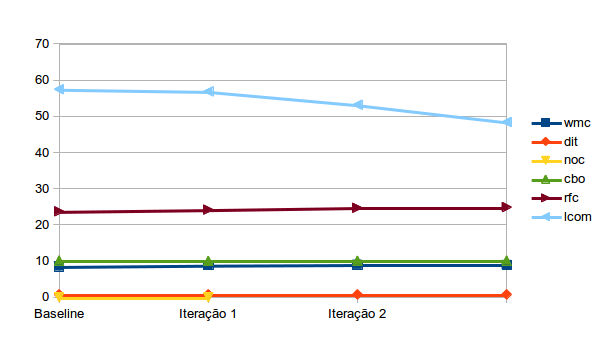
\includegraphics{img/allmetrics}
	\end{center}
	\legend{Fonte: Próprio Autor}
\end{figure}


É possível observar nos resutados a relação entre LCOM e as métricas 
WMC,RFC que aumentaram conforme o LCOM diminuia. O aumento da complexidade
indicado pelas métricas WMC e RFC é pequeno em comparação ao aumento de
coesão indicada pela métrica LCOM. Pode-se chegar a essa conclusão, não somente
analisando os resultados, como também ao analisar o código em que as classes
estão menores, mais coesas, com responsabilidades bem definidas. Portanto, a
arquitetura proposta melhorou a qualidade do objeto de estudo porque promoveu
maior coesão e diminuiu a complexidade.

A maioria das métricas tendem a aumentar durante o processo de refatoração. 
É válido resaltar que as três classes refatoradas são as mais complexas do
pacote de grupos com valores anômalos para as métricas. Portanto, somente após
uma refatoração em uma amostragem maior de classes que se é possível determinar
um valor limite para as métricas, inclusive para um projeto construído do zero.
Com os dados coletados durante o desenvolvimento é possível definir
esses valores limites para identificar anomalias nas classes e tratar cada caso
isolado.

 
\section{Trabalhos Futuros}

Existem outros padrões de projetos para o desenvolvimento da camada de
apresentação de um software que não foram analisados nesse trabalho, a saber: 
MVVM, MVP-VM, MVPC. Essas variações no padrão MVC surgiram em contextos
diversificados e podem agregar algum benefício à qualidade do aplicativo.
Este trabalho não aborda o impacto do padrão MVP em outras métricas de qualidade
de código derivadas do CK.
Não foi feita uma avaliação dos impactos na performance do aplicativo devido ao
uso do padrão MVP. A inclusão de mais objetos interagindo trocando mensagens
pode depreciar a performance, levando-se em consideração sua execução em
ambientes mais restritos, como no caso de um aparelho móvel.